\thispagestyle{empty}
\begin{center}
  \normalfont\sffamily\bfseries

  {\LARGE Zeta-values of arithmetic schemes\\
    at negative integers\\
    and Weil-étale cohomology

  }

  \vspace{\fill}

  Proefschrift\\
  ter verkrijging van\\
  de graad van Doctor aan de Universiteit Leiden\\
  op gezag van Rector Magnificus prof. mr. C.J.J.M. Stolker,\\
  volgens besluit van het College voor Promoties\\
  te verdedigen op maandag 10 december 2018\\
  klokke 12:30 uur

  \vspace{\fill}

  door

  \vspace{\fill}

  Alexey Beshenov\\
  geboren te Lipetsk, USSR, in 1989
\end{center}

\newpage

\thispagestyle{empty}

\noindent \textbf{Promotor}: Prof. dr. Baptiste Morin (Université de Bordeaux) \\
\noindent \textbf{Promotor}: Prof. dr. Sebastiaan J. Edixhoven

\vspace{2em}

\noindent\textbf{Samenstelling van de promotiecommissie:}

\noindent Prof. dr. Stephen Lichtenbaum (Brown University, USA) \\
Prof. dr. Niranjan Ramachandran (University of Maryland, USA) \\
Prof. dr. Peter Stevenhagen \\
Prof. dr. Aad van der Vaart

\vspace{\fill}

\begin{center}
  \noindent This work was funded by Erasmus Mundus ALGANT DOC program\\
  and was carried out at Université de Bordeaux and  Universiteit Leiden

  \vspace{1em}

  \noindent\raisebox{+0.125cm}{
\includegraphics[width=2.5cm]{u-bordeaux.pdf}}\hspace{0.9cm}
  \raisebox{+0.12cm}{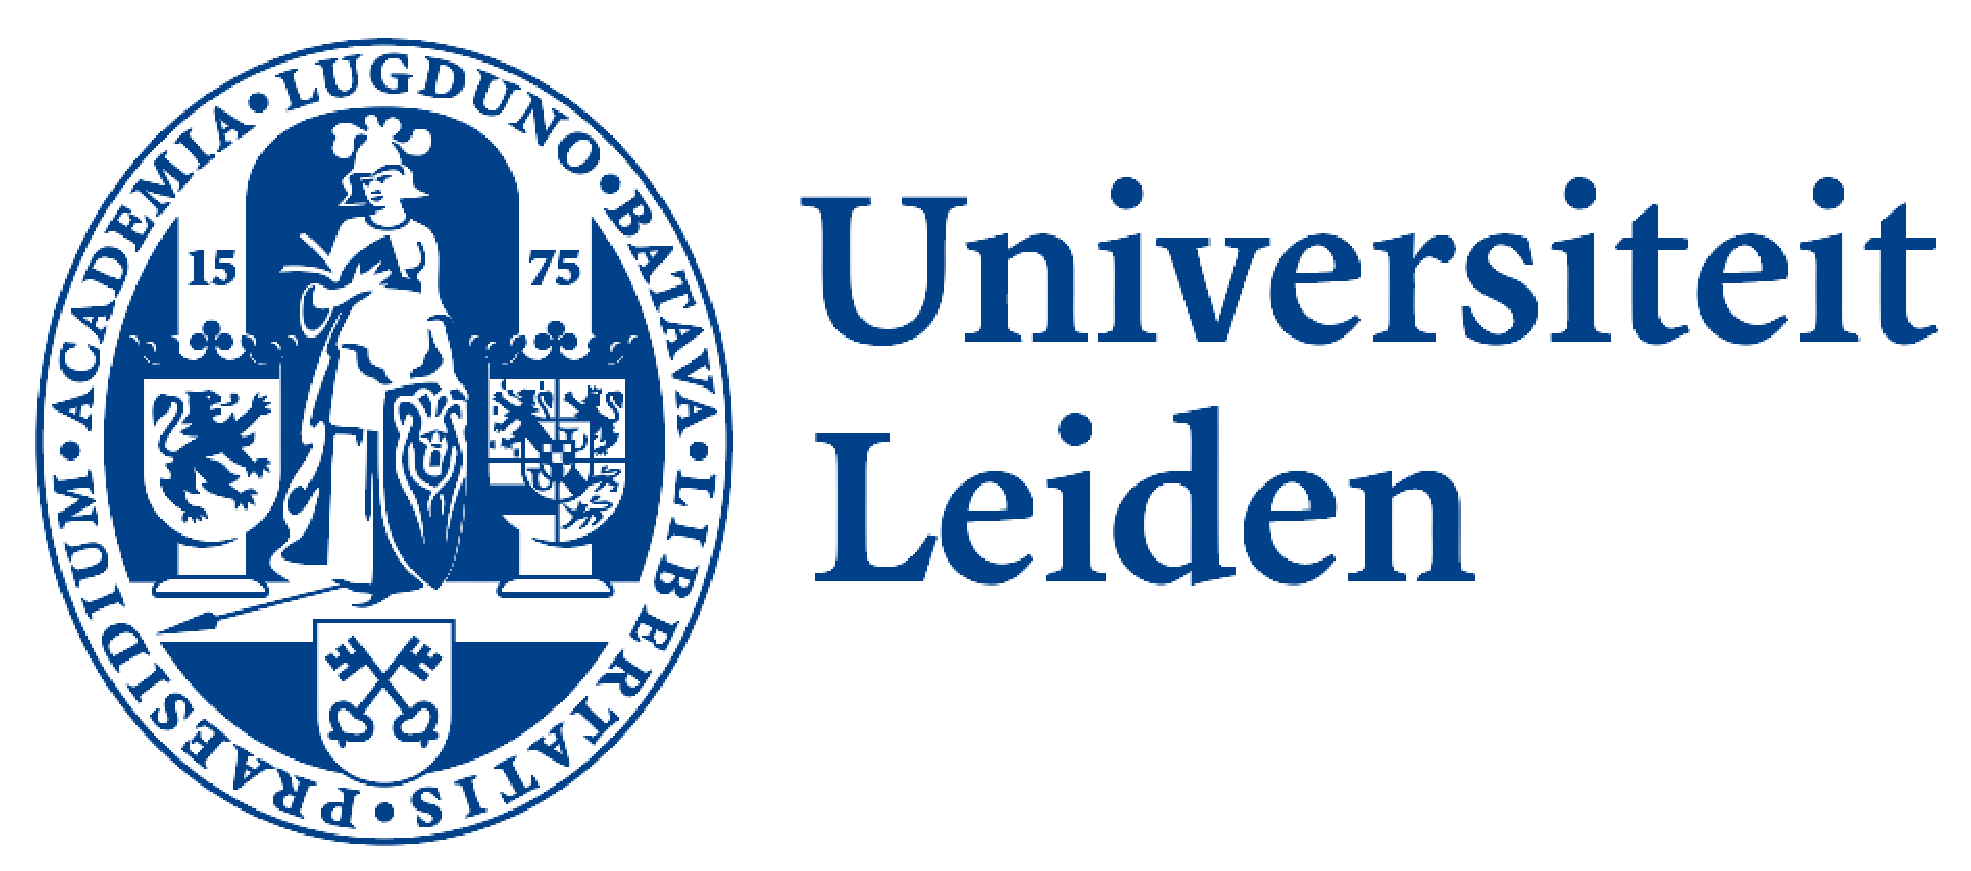
\includegraphics[width=2.25cm]{leiden.pdf}}\hspace{0.9cm}
  \includegraphics[width=2.5cm]{algant.mps}
\end{center}
